\subsection{Unsupervised Learning}
While supervised learning aims to entangle patterns by examining data that has been labeled by humans, unsupervised learning attempts to do the same with unlabeled data. This requires algorithms that can examine unstructured information and find commonalities and dissimilarities between data points. Humans are exceptional at unsupervised learning, performing tasks of separation and discrimination from a young age. For example, children "can discriminate faces and voices by sex, habituate to faces of both sexes, and make inter-modal associations between faces and voices" \cite{martin2010patterns}. These skills to separate items based on patterns are also evident in our everyday lives: we separate tasks into work, pleasure, or home-related categories; cars into new, old, attractive, or boring; restaurants into lower-end (e.g. McDonalds) or high-end (e.g. Red Lobster); people into races. In most if not all of the previous cases, we are not \textit{told} what items belong to what categories, and in fact we are not told what the categories are. Rather, we assume that there are some categories, and we attempt to distribute items into the categories that make the most sense to us. This human ability to discern patterns from unstructured data is similar to how unsupervised learning works.

With most unsupervised learning algorithms, the number of categories is known or guessed, and it is the job of the algorithm to separate the data into that many categories in the best possible way. A plethora of unsupervised learning algorithms exist, most of which are extensions on more basic and fundamental ones. Some of the fundamental algorithms include K-means clustering, fuzzy clustering, single linkage clustering, self organized maps, and vector quantization. For the purposes of this work, we only cover the simple K-means algorithm, an extension of which we use in the experimental section of this paper.

\subsubsection{K-means Clustering}
K-means clustering is a powerful tool used in various fields mainly for cluster analysis. It operates on basic principles of finding subsets of data that share the most commonality between one another. This algorithm requires the data to be in continuous numerical form, and uses one of several measures of distance to attribute closeness. The most widely used measure of distance is the Euclidean distance 
$$
D(x, y) = \sqrt{(x_1 - y_1)^2 + (x_2 - y_2)^2 + \dots + (x_n - y_n)^2}.
$$
K-means works by finding $k$ centers of clusters, where $k$ is the number of hypothesized clusters given by the user. This goal is achieved by first choosing $k$ random points from all the points in the given dataset. All the remaining points are then matched with the closest center, and each matched set of points is declared as a cluster. For centers $c_1, c_2, \dots, c_n$ and point $x$, $x$ belongs to the cluster whose center is the closest to $x$ 
$$
Cluster(x) = \arg \min_{c} \Big( D(c_1, x), D(c_2, x), \dots, D(c_k, x) \Big).
$$
Once all the points have been assigned to a cluster, an approximate center point of each cluster is calculated as the mean of all the points in that cluster
$$
\hat c_i = mean(x_{i,1}, x_{i,2}, \dots, x_{i,l})
$$
where $x_{i,j}$ is the $j^{th}$ point in the $i^{th}$ cluster.
A new center for the cluster, $c_i$, is then chosen, with the new center being the closest to the approximate center point
$$
c_i = \arg \min_{x} \Big( D(\hat c_i, x_{i, 1}), D(\hat c_i, x_{i, 2}), \dots, D(\hat c_i, x_{i, 2}) \Big ) .
$$
This will result in a change of points-to-cluster-center distances, and will therefore change the clusters that some points belong to, which will change the cluster centers, resulting in a cycle of improvement that has been proven to converge with the repetition of the center assignment steps (Fig. \ref{fig:k-means}). While the K-means algorithm is useful in its own right, extensions have made it more powerful. An example of such an extension is the Gaussian Mixture model, which is a more generalized form of the K-means that assumes there are $k$ uniform distributions with unknown parameters. This generalization allows the model to group clusters using several covariance shapes, meaning the distance relationships are much more diverse and flexible (Fig. \ref{fig:gaussian_mixture}) .

% \begin{figure}[!h]
%   \centering
%   \begin{subfigure}{.3\textwidth}
%     \centering
%     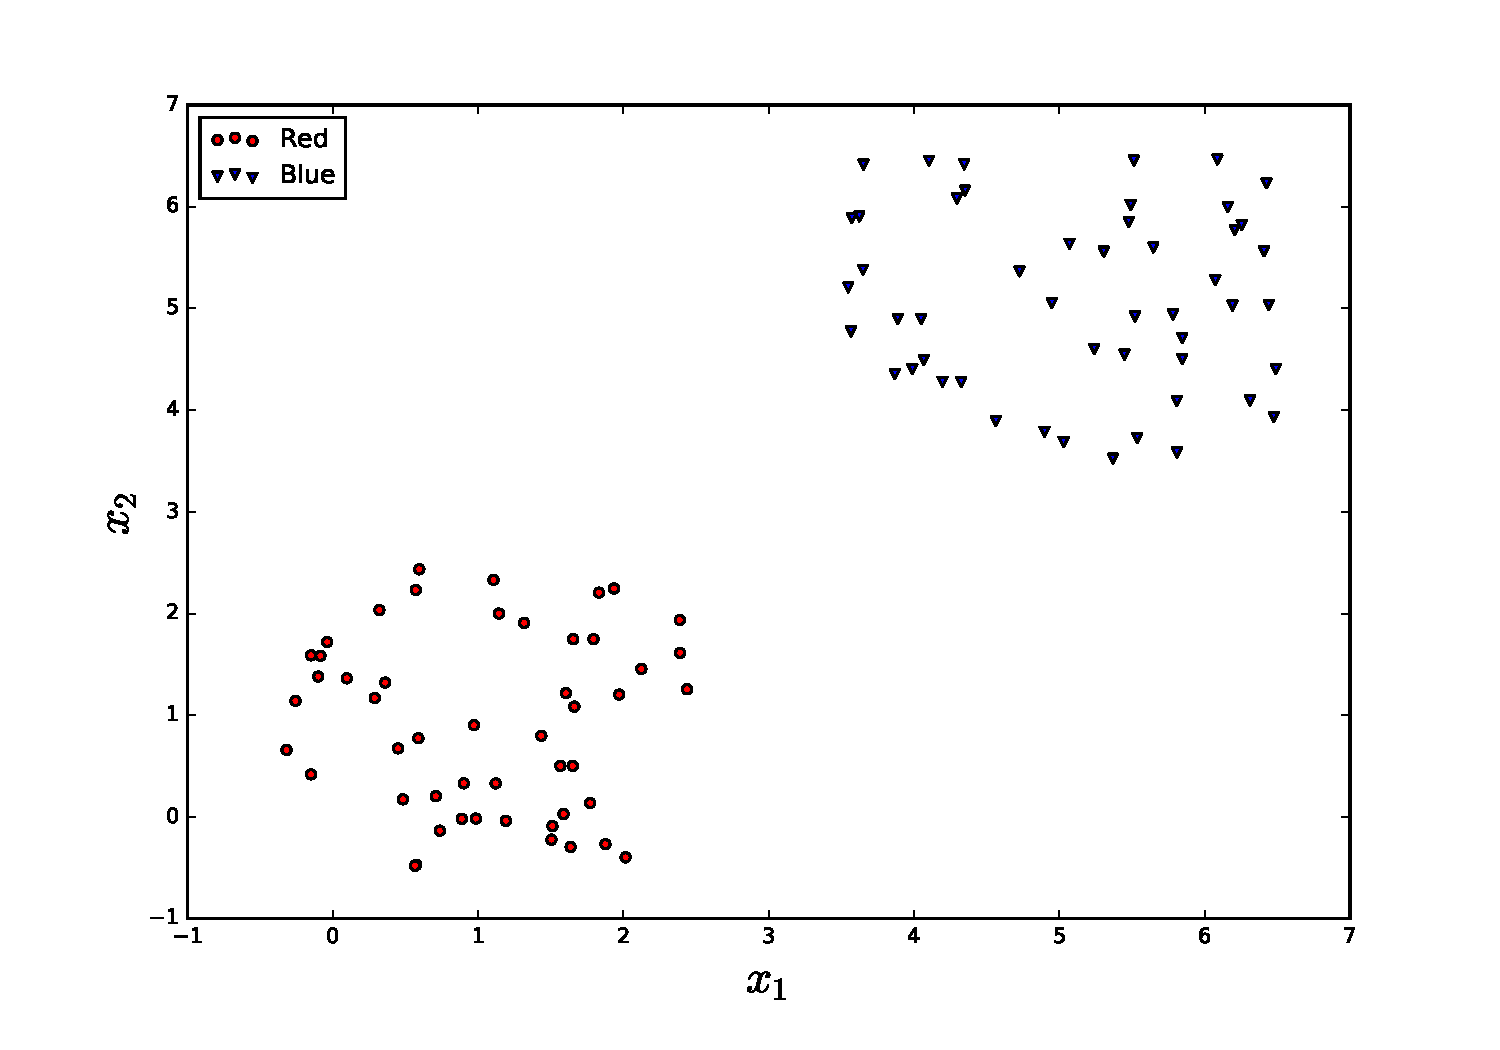
\includegraphics[width=\linewidth]{figures/twoClasses_separable.pdf}
%   \end{subfigure} %
%   \begin{subfigure}{0.3\textwidth}
%     \centering
%     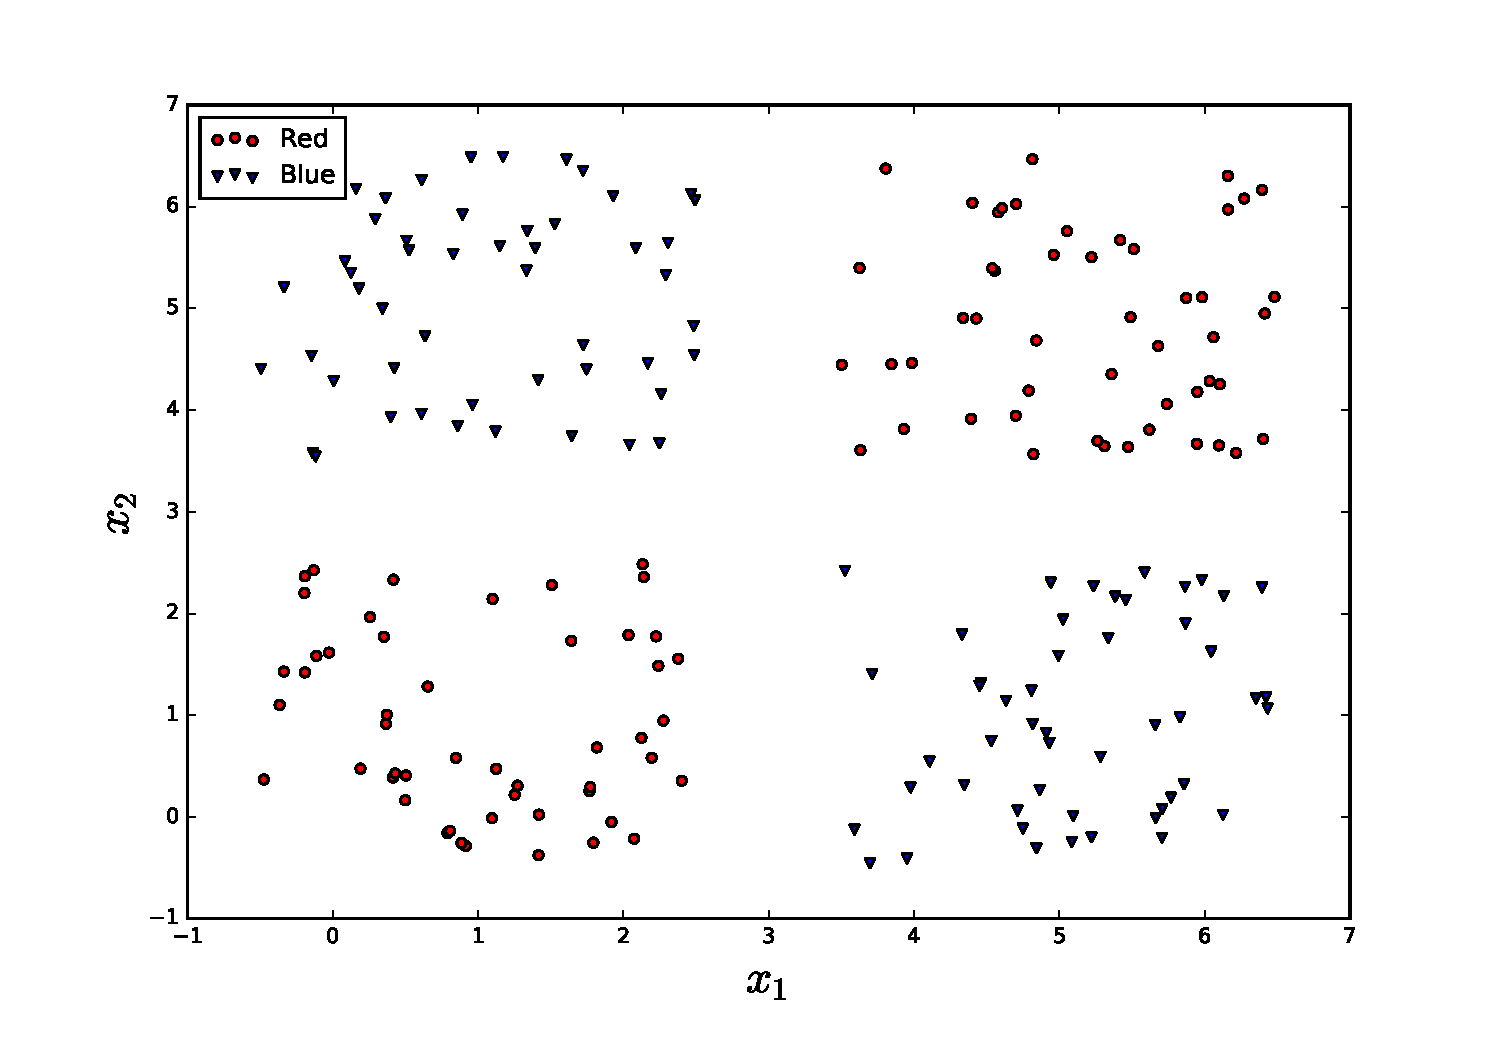
\includegraphics[width=\linewidth]{figures/twoClasses_non_separable.pdf}
%   \end{subfigure}
% 	\begin{subfigure}{0.3\textwidth}
% 		\centering
% 		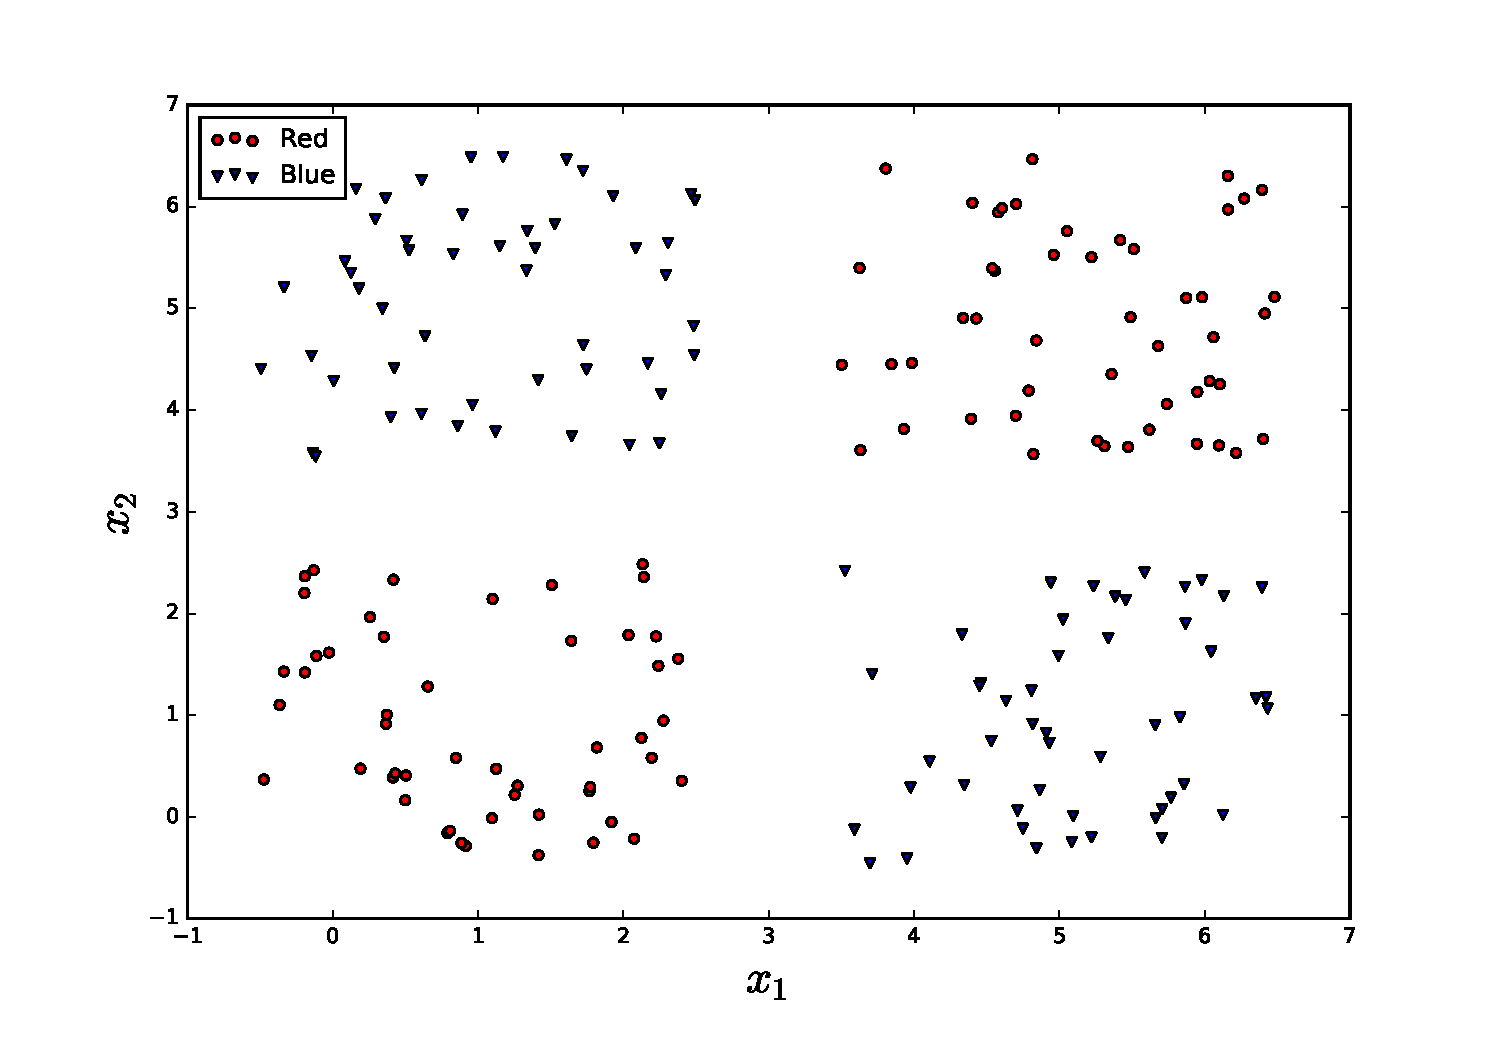
\includegraphics[width=\linewidth]{figures/twoClasses_non_separable.pdf}
% 	\end{subfigure}
%   \caption{Two sets of data, one of which is linearly separable (Left) and the other is non linearly separable (Right). Linear separability means that a line can be found that can perfectly segregate the two classes into two sections. A diagonal, horizontal, or vertical line between the blue and red points can be drawn on the left that achieves that goal. However, on the right there is no one line that can be used to separate the red from blue points. This problem of finding a line of separation between two linearly separable data sets can be solved by using a binary classifier, the earliest example of which is the perceptron.}
%   \label{fig:two_classes_example}
% \end{figure}
